\subsection{Evolution System}

The formulation employed in this chapter was initially developed and published in Ref.~\cite{PhysRevD.96.104040}. Although the primary focus of that publication differs from the subject matter of this chapter, Appendix A of the paper contains the 3+1 decomposed Klein-Gordon equation for a massive scalar field, as presented in equations A3c and A3d. For the sake of completeness, these equations are
%
\begin{align}
  \partial_t \Phi =   & -2 \alpha K_\phi + \mathcal{L}_\beta \Phi \label{eq:wave_scattering_a3c}                                                                                                                                                     \\
  \partial_t K_\Phi = & \alpha \left( K K_\Phi - \frac{1}{2} \gamma^{ij} D_i \partial_j \Phi + \frac{1}{2} \mu^2 \Phi \right) - \frac{1}{2} \gamma^{ij} \partial_i \alpha \partial_j \Phi + \mathcal{L}_\beta K_\Phi, \label{eq:wave_scattering_a3d}
\end{align}
%
where $\Phi$ is the scalar field being evolved, $K_\Phi$ its ``canonical momentum'', given by
%
\begin{equation}
  K_\Phi = -\frac{1}{2\alpha} \left( \partial_t - \mathcal{L}_\beta \right)\Phi,
  \label{eq:wave_scattering_a2}
\end{equation}
%
$\alpha$ is the spacetime lapse, $\beta^i$ its shift vector, $\gamma^{ij}$ its induced 3-metric, $K$ the trace of its extrinsic curvature tensor, $D_i$ the covariant derivative associated with $\gamma^{ij}$, $\mu$ the spacetime mass parameter and $\mathcal{L}_\beta$ is the Lie derivative along the shift vector $\beta^i$, given explicitly by
%
\begin{equation}
  \mathcal{L}_\beta\Phi = \beta^i \partial_i \Phi.
  \label{eq:wave_scattering_lie_derivative}
\end{equation}

To expand each component of these equations, we utilized the mathematical software package \texttt{Wolfram Mathematica}. The resulting expansion was subsequently implemented into the \texttt{Thorn} by automatically generating corresponding \texttt{C} code from within \texttt{Mathematica}. The code used in this process can be found in \texttt{Notebooks/equations.nb} of the \texttt{Thorn}'s repository.

\subsection{Initial data}

The implementation supports three distinct initial conditions for the scalar field and its canonical momentum. These include a plane wave, an exact Gaussian, and a multipolar Gaussian function. The plane wave and exact Gaussian initial data were developed for the purpose of testing multipatch derivatives in flat spacetime, which will be elaborated on further in subsequent sections. The exact Gaussian initial data is named as such to reflect the fact that it is an exact solution of the Klein-Gordon equation in flat spacetime.

The multipolar Gaussian function is a basic Gaussian function that is multiplied by a linear combination of real spherical harmonics. This particular function was the one chosen during our ``production'' runs as it has the ability to excite specific modes in the system based on the chosen parameters for the linear combination. The development of this initial data is based on the methodology presented in Ref.~\cite{PhysRevD.87.043513}. In order to construct it, let us first introduce its components. We start with the Gaussian function $G(r, \sigma)$, given by
%
\begin{equation}
  G(r, \sigma) = \exp\left( -\frac{1}{2} \left( \frac{r}{\sigma} \right)^2  \right).
  \label{eq:wave_scattering_gaussian}
\end{equation}
%
where $\sigma$ is the Gaussian width parameter. Next, we introduce the real spherical harmonics $Y_{lm}(x,y,z)$, given by
%
\begin{equation}
  Y_{lm}(x, y, z) =
  \begin{cases}
    A_{lm} P_{lm}\left( \frac{z}{\sqrt{x^2 + y^2 + z^2}} \right) \cos(m \arctan(y,x)) \text{ if } m \geq 0  \\
    A_{lm} P_{l|m|}\left( \frac{z}{\sqrt{x^2 + y^2 + z^2}} \right) \sin(|m| \arctan(y,x)) \text{ if } m < 0 \\
  \end{cases}
  ,
  \label{eq:wave_scattering_real_spherical_harmonics}
\end{equation}
%
where $P_{lm}(x)$ are the associated Legendre polynomials and the $A_{lm}$ coefficients are given by
%
\begin{equation}
  A_{lm} = (-1)^m \sqrt{\frac{2 l + 1}{4\pi} \frac{(l-m)!}{(l+m)!}}.
  \label{eq:wave_scattering_real_spherical_harmonics_coeffs}
\end{equation}
%
By introducing ``shifted coordinates''
%
\begin{align}
  X & \equiv x - x_0 \label{eq:wave_scattering_real_spherical_harmonics_shifted_x}                \\
  Y & \equiv y - y_0 \label{eq:wave_scattering_real_spherical_harmonics_shifted_y}                \\
  Z & \equiv z - z_0 \label{eq:wave_scattering_real_spherical_harmonics_shifted_z}                \\
  R & \equiv \sqrt{X^2 + Y^2 + Z^2} \label{eq:wave_scattering_real_spherical_harmonics_shifted_r} \\
\end{align}
%
it is possible to shift the location of the center of the function to $(x_0,y_0,z_0)$. Combining these pieces, the multipolar Gaussian function $M_G(x,y,z)$ is written as
%
\begin{equation}
  M_G(x, y, z) = \sum_{l=0}^{N}\sum_{m = -l}^{l} c_{l m} Y_{l m}(X,Y,Z) G(R-R_0,\sigma)
  \label{eq:wave_scattering_multipolar_gaussian}
\end{equation}
%
where $R_0$ is the radius of the Gaussian function. Once again, code generation routines for the initial data can be found in \texttt{Notebooks/equation.nb}. It is important to note that in the implemented code, the series is expanded up to $N = 2$, and higher multipole orders are not supported.

Figure~\ref{fig:multipolar_gaussian_id_demo} showcases three distinct configurations of the multipolar Gaussian function. For all panels, the parameters $x_0$, $y_0$, and $z_0$ were assigned a value of zero, while $R_0$ was set to 5. Panel \textbf{A} displays a plot where $c_{00}$ is assigned a value of $1/A_{00}$, and all other coefficients are set to zero. In Panel \textbf{B}, $c_{11}$ is set to $1/A_{11}$, and all other coefficients are set to zero. Finally, in Panel \textbf{C}, $c_{22}$ is assigned a value of $1/(3A_{22})$, and all other coefficients are set to zero.

\begin{figure}[!ht]
  \centering
  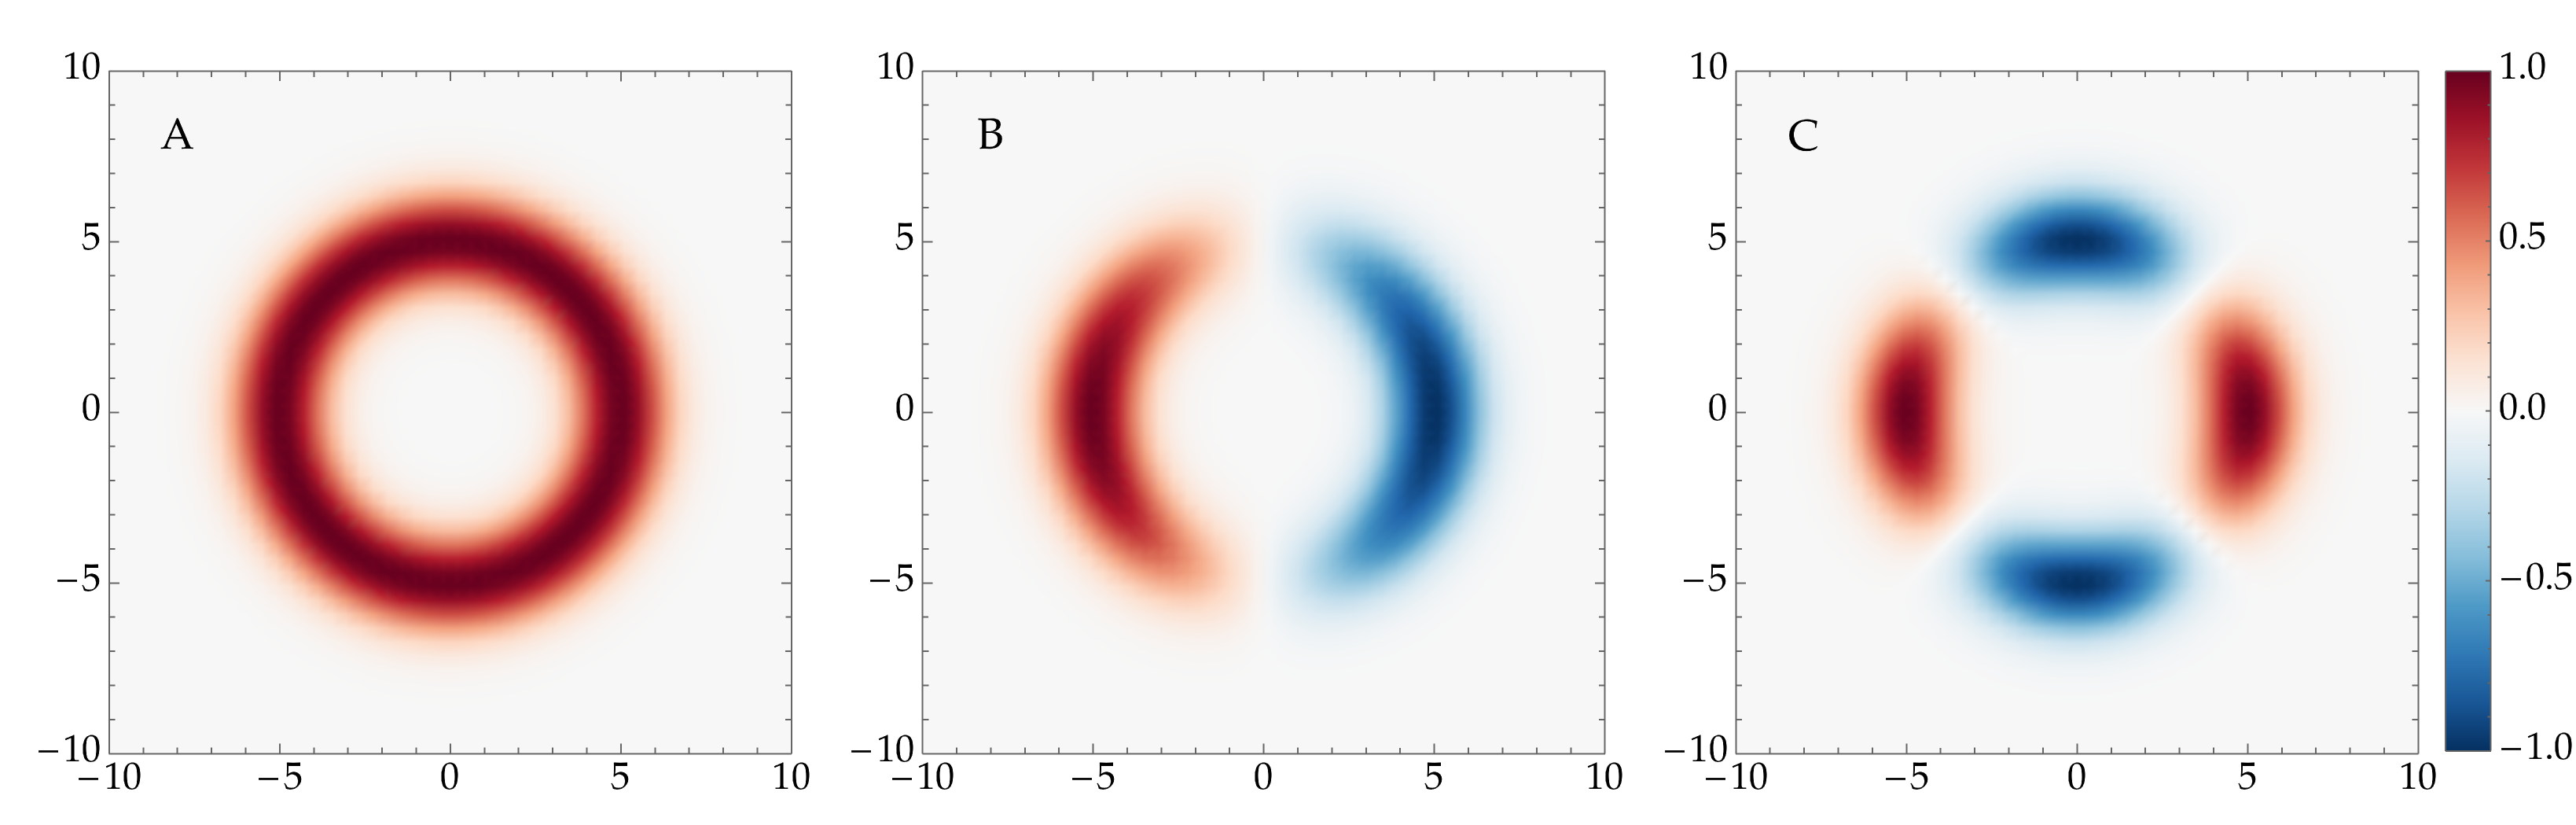
\includegraphics[width=\linewidth]{img/wave_scattering/multipolar_gaussian_id_examples.png}
  \caption{Demonstration of the multipolar Gaussian function with different parameters. For all panels, $x_0 = y_0 = z_0 = 0$ and $R_0 = 5$. In Panel \textbf{A} displays the only nonzero coefficient is $c_{00} = 1/A_{00}$, in Panel \textbf{B}, $c_{11} = 1/A_{11}$, and in Panel \textbf{C}, $c_{22} = 1/(3A_{22})$.}
  \label{fig:multipolar_gaussian_id_demo}
\end{figure}

\subsection{Evolution Code}

The coordinate system used in our grid setup was the \texttt{Thornburg04} coordinates, implemented through the \texttt{Llama}~\cite{PhysRevD.83.044045} infrastructure. This coordinate system comprises spherical wedges, each covering 90 degrees in all three dimensions, and centered on the $+x$, $-x$, $+y$, $-y$, $+z$, and $-z$ axes. These wedges provide complete coverage of a region between $r_\text{min}$ and $r_\text{max}$, with smooth inner and outer boundaries, and a cubical patch enclosing $r < r_\text{min}$ where standard \texttt{Carpet}~\cite{Schnetter:2003rb} box-in-box mesh refinement can be applied.

To set up the gravitational initial data, we used \texttt{TwoPunctures}~\cite{Ansorg:2004ds} with parameters that emulate the GW150914 merger. Gravitational evolution was performed using \texttt{ML\_BSSN}~\cite{Brown:2008sb,Kranc:web,McLachlan:web} with a $1+\log$ slicing condition and a $\Gamma$-driver shift. We employed 7 levels of mesh refinement boxes via \texttt{Carpet}, centered around each of the punctures and tracking their motion via \texttt{PunctureTracker}. We developed the \texttt{KleinGordon Thorn}, which we describe in this section, to evolve a massless scalar field with initial data provided by a multipolar Gaussian function, centered around the origin with $R_0 = 15.0$, width $\sigma = 1.0$, and the only non-zero multipolar coefficient being $c_{00} = 1 / A_{00}$. This spherically symmetric initial data allowed us to activate reflection symmetry around the $+z$ plane in the code, which saved computational time, memory, and storage space.

In the gravitational evolution code, spatial derivatives were provided by \texttt{SummationByParts}~\cite{Diener:2005tn}, which provides finite difference stencils satisfying the summation-by-parts property with embedded Kreiss-Oliger type artificial dissipation. In \texttt{KleinGordon}, we utilized handcrafted central finite difference stencils and added artificial Kreiss-Oliger dissipation to the evolved Klein-Gordon fields via \texttt{Dissipation}. The gravitational evolution code projected its derivative operators into the global coordinate system utilized by \texttt{Llama} via \texttt{GlobalDerivative}, but in \texttt{KleinGordon}, this projection was also handcrafted via the Jacobian and Jacobian derivative components provided by \texttt{Llama}. Code generation for these projections can be found in the \texttt{Notebooks/equations.nb} notebook. Both evolutions utilized 8th order finite difference stencils, and radiating boundary conditions were employed in the outer boundaries via \texttt{NewRad}.

The time integration scheme utilized in this study was method of lines, provided by the \texttt{MoL Thorn}. A 4th order Runge-Kutta method with fixed time step was employed for the time integration process. It is important to note that \texttt{Carpet} employs different time steps for various refinement levels, thus the time step specified in the parameter files pertains to the coarsest level. The final integration time was selected in conjunction with the outer boundary radius to minimize interference from reflections at the outer boundaries, inter-patch boundaries, and inter-refinement level boundaries on the scalar field signal being measured.

At regular time intervals, data was extracted at $7$ different radii using \texttt{Multipole}, as well as 2D and 3D field data evolved by \texttt{KleinGordon}. Additionally, statistics such as puncture locations were recorded, which enabled the construction of visualizations of the simulated data. These results will be presented shortly. The parameter file used for this evolution can be located in the specified GitHub repository under \texttt{KleinGordon/par/GW150914/GW150914\_Scalar\_field.par}.

\subsection{Results}

The results depicted in Figure~\ref{fig:wave_scattering_results} illustrate the scattering of the scalar field $\Phi$ by the GW150914 binary black hole merger system at three distinct moments in time. Panel \textbf{A} corresponds to $t = 0$, panel \textbf{B} represents $t = 8.811$, and panel \textbf{C} corresponds to $t = 55.068$. Following the initial interaction, the black holes generate a wavefront in a pattern resembling a cardioid, where the cusp coincides with the hole location and propagates in alternating directions. This shape is identical to that observed in wave scattering by a single black hole, however, in the case of a merging binary, we can observe clear effects arising from the rotation of the holes and interference from the waves produced by each. An animation of the scattering process can be viewed \href{https://github.com/lucass-carneiro/phd-thesis/tree/main/img/wave_scattering/scattering.gif}{here}.

%Frames used: 0 7 19
\begin{figure}[h]
  \centering
  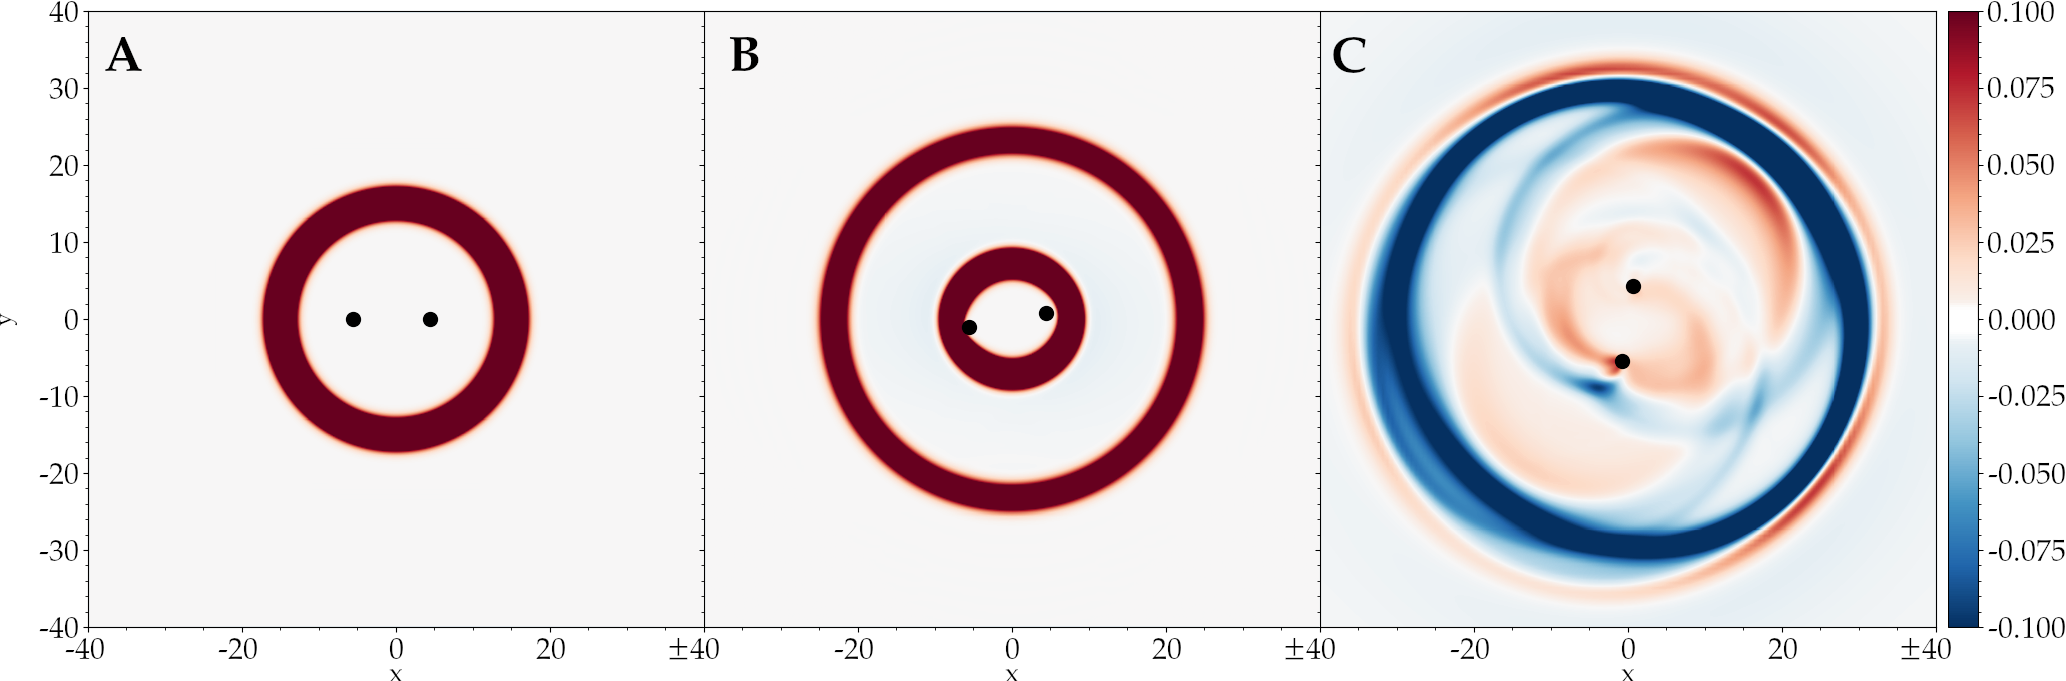
\includegraphics[width=\linewidth]{img/wave_scattering/scattering_frames}
  \caption{Scalar field $\Phi$ scattering of the GW150914 binary merger in three moments in time. Panel \textbf{A} corresponds to $t = 0$, panel \textbf{B} represents $t = 8.811$, and panel \textbf{C} corresponds to $t = 55.068$.}
  \label{fig:wave_scattering_results}
\end{figure}